		\subsection{Statistical Mixtures and Density Operator}

			If only the subsystem of a pure quantum state is accessible to measurements, or the state of the system is not known at the microscopic level (statistical ensemble!), the state of the system has to be described by a Hermitian density operator
			%
			\begin{align}
				\Aboxed{\hat{\rho} = \sum_{n=1}^N p_n \ket{\phi_n}\bra{\phi_n}.}
			\end{align}
			Here, $\bra{\phi_n}$ are the eigenstates of $\hat{\rho}$, and $p_n$ are the probabilities to find the system in the respective states $\ket{\phi_n}$.

			Let us now have a brief look at the properties of the density operator:
			\begin{itemize}
				\item The trace of the density operator is the sum of all probabilities $p_n$:
				%
				\begin{align}
					\tr{\rhohat} = \sum p_n = 1.
				\end{align}
				%
				\item For a pure state $\ket{\psi}$, we get $p_n=1$ for only one value of $n$. For every other $n$, the probabilities vanish. We thus obtain a ``pure'' density operator $\rhohat_{\text{pure}}$ which has the properties of a projection operator:
				%
				\begin{align}
					\rhohat_{\text{pure}} = \ket{\psi}\bra{\psi} \qquad \Longleftrightarrow \qquad \rhohat^2 = \rhohat.
				\end{align}
			\end{itemize}
			%
			With this knowledge we can now determine the result of a measurement of an observable $A$ belonging to an operator $\hat{A}$. For the pure state $\ket{\psi}$ we get:
%
			\begin{align}
				\bra{\psi} \hat{A} \ket{\psi}.
			\end{align}
			%
			For a mixed state we get:
			%
			\begin{align}
				\tr{\rhohat \cdot \hat{A}} = \sum_n {p_n} \bra{\phi_n} \hat{A} \ket{\phi_n}.
			\end{align}
			The time evolution of the density operator can be expressed with the von Neumann equation:
			\begin{align}
				i\hbar \diff{}{t}\rhohat(t) = [\hat{H}(t),\rhohat(t)].
			\end{align}
				\paragraph{Example.} 
					If we consider a system $S = S_1 \otimes S_2$ comprised of two subsystems $S_1$, $S_2$, then the density operator $\hat{\rho}_i$ of  subsystem $i$ is
					%
					\begin{align}
						\rhohat_1=&\trarb{2}{\rhohat},\\
						\rhohat_2=&\trarb{1}{\rhohat},
					\end{align}
					%
					where $\hat{\rho}=\ket{\psi}\bra{\psi}$ and $\trarb{j}{\rhohat}$ is the trace over the Hilbert space of subsystem $j$ (cf. first tutorial).
					%\\
					%\rhohat_2=\trarb{2}{\rhohat}
		\subsection{Important Consequences of the Principles}

			\subsubsection{Uncertainty Relation}
				The product of the variances of two noncommuting operators has a lower limit:
				\begin{align}
					\Delta \hat{A} \cdot \Delta \hat{B} \geq \frac{1}{2} \left| \Braket{\left[\hat{A},\hat{B}\right]} \right|,
				\end{align}
				where the variance is defined as $\Delta \hat{A} = \sqrt{\Braket{\hat{A}^2}-\Braket{\hat{A}}^2}$.

				\paragraph{Examples.}
					\begin{align}
						\left[ \hat{x}, \hat{p} \right] &= i \hbar \\
						\left[ \hat{J}_i , \hat{J}_j \right] &= i \hbar \epsilon_{ijk} \hat{J}_k
					\end{align}
				\paragraph{Note.} This is a statement about the \emph{state} itself, and not the measurement!

			\subsubsection{Ehrenfest Theorem}
				With the Ehrenfest theorem, one can determine the time evolution of the expectation value of an operator $\hat{A}$:
				\begin{align}
					\diff{}{t}\Braket{\hat{A}}=\frac{1}{i\hbar}\Braket{\left[\hat{A},\hat{H}\right]}+\Braket{\diffp{\hat{A}}{t}}. \label{eq:ehrenfest}
				\end{align}
				%
				If $\hat{A}$ is time-independent and $\left[\hat{A},\hat{H}\right]=0$, the expectation value $\Braket{\hat{A}}$ is a constant of the motion.

	\section{Motion of a Point-Like Particle}
		\subsection{Wave Functions}
			In the following, we consider a point-like particle and its observables $\vv{r}$ and $\vv{p}$. The possible basis states can be constructed from the observables we measure. We thus get $\ket{\vv{r}}$ and $\ket{\vv{p}}$ as basis states. Since the particle is localized at one point, we get
			\begin{align}
				\braket{\vv{r}|\vv{r}'} =\delta(\vv{r}-\vv{r}').
			\end{align}
			%
			With the completeness relation, we can express the wave function $\ket{\psi}$ of the particle as a linear combination of all possible position states $\ket{\vv{r}}$:
			\begin{align}
				\ket{\psi}=\int \dif \vv{r} \ket{\vv{r}}\braket{\vv{r}|\psi},
			\end{align}
			where $\psi(\vv{r})=\braket{\vv{r}|\psi}$ and $\psi^*\psi$ is the probability density.
			%
			The eigenstates of $\hat{\vv{p}}$ are
			\begin{align}
				\ket{\vv{p}}&=\int \dif \vv{r} \ket{\vv{r}} \braket{\vv{r}|\vv{p}} \\
				&= \frac{1}{(2\pi\hbar)^{\frac{3}{2}}} \int \dif \vv{r} \eexp{{i \vv{p}\cdot\vv{r}}/{\hbar}}\ket{\vv{r}},
			\end{align}
			where the exponential function in the integral can be interpreted as a plane wave.
			%
			If we expand $\ket{\psi}$ in terms of $\ket{p}$, we get
			\begin{align}
				\ket{\psi}=\int \dif \vv{p} \ket{\vv{p}}\underbrace{\braket{\vv{p}|\psi}}_{=\phi(\vv{p})}.
			\end{align}
			The second factor in the integral can be expanded as follows:
			\begin{align}
				\phi(\vv{p})	&=\braket{\vv{p}|\psi}\\
				&=\int\dif\vv{r}\braket{\vv{p}|\vv{r}}\braket{\vv{r}|\psi}\\
				&=\frac{1}{(2\pi\hbar)^{\frac{3}{2}}} \int\dif\vv{r}\eexp{-i\vv{p}\cdot\vv{r}/{\hbar}}\psi(\vv{r}) \label{eq:fourier}
			\end{align}
			Equation \eqref{eq:fourier} shows that $\phi(\vv{p})$ and $\psi(\vv{r})$ are Fourier transforms of each other.

	\subsection{Translations of $\ket{\psi}$ in Time, Space and Momentum}

		\subsubsection{Time: Schrödinger Equation}
			In the following, we would like to get a basic intuition of how quantum mechanics works. For the Schrödinger equation
			\begin{align}
				i\hbar \diffp{\ket{\psi(t)}}{t} = \hat{H}\ket{\psi(t)} \label{eq:schrodinger2}
			\end{align}
			we get the formal solution
			\begin{align}
				\ket{\psi(t)}=\hat{U}(t,0)\ket{\psi(0)}, \label{eq:psit}
			\end{align}
			where
			\begin{align}
				\hat{U}(t,0) = \eexp{-i{\hat{H}t}/{\hbar}} \label{eq:timeevolutionoperator}
			\end{align}
			is the time evolution operator. If we write out the Hamiltonian of the point-like particle in \eqref{eq:schrodinger2}, we get
			\begin{align}
				i\hbar \diffp{\psi(\vec{r},t)}{t} = -\frac{\hbar^2}{2m}\Laplace\psi(\vv{r},t)+V(\vv{r},t)\psi(\vv{r},t).
			\end{align}
			The wave function $\psi(\vec{r},t)$ at time $t$ can be determined with the help of \eqref{eq:psit} and \eqref{eq:timeevolutionoperator}:
			\begin{align}
				\psi(\vv{r},t)	&=\braket{\vv{r}|\psi(t)}=\braket{\vv{r}|\hat{U}(t,0)|\psi(0)}\\
				&=\int\dif\vv{r}'\bra{\vv{r}}\hat{U}(t,0)\overunderbraces{&\br{2}{\mathbb{1}}}{&\ket{\vv{r}'}&\bra{\vv{r}'}&\psi(0)\rangle}{&&\br{2}{\psi(\vv{r}',0)}}.
			\end{align}
			% 
			%\overunderbraces{&\br{2}{a}}{&&}{&&\br{2}{}}
			The first factor in the integral describes the propagation of a wave packet localized at $\vv{r}'$ during the time $t$. The second factor is the wave function of a particle localized at $\vv{r}'$ at a time $t=0$. %Is wave function of particle?

			\subsubsection{Space and Momentum}

				Just like $\hat{H}$ is a generator of translation in time, $\hat{\vv{p}}$ is the generator for translation in space and $\hat{\vv{r}}$ is the generator for translation in momentum:
				\begin{align}
					\hat{\mathcal{T}}_R(\Delta{\vv{r}}) \ket{\vec{r}} &= \eexp{-i\hat{\vv{p}}\cdot{\Delta\vv{r}}/{\hbar}}\ket{\vv{r}}=\ket{\vv{r}+\Delta\vv{r}},\\
					\hat{\mathcal{T}}_R(\Delta{\vv{p}}) \ket{\vec{p}} &= \eexp{-i\hat{\vv{r}}\cdot{\Delta\vv{p}}/{\hbar}}\ket{\vv{p}}=\ket{\vv{p}+\Delta\vv{p}}.
				\end{align}


\marginpar{\scriptsize{Lecture 3}}
	\section[The Two-Level System]{The Two-Level System\footnote{cf. \cite{cohen}, chapter 4}}

		There are many examples for two-level systems that can be found in nature:
		\begin{itemize}
			\item Spin of the electron: Up vs. down state
			\item Two-level atom with one electron (simplified): Excited vs. ground state
			\item Structures of molecules, e.g., \hyperref[fig:twostate]{\ch{NH3}}
		\end{itemize}
		Two-level systems are also used excessively in information technology.
		How do we induce dynamics, i.e., population transfer between the two levels $\ket{1}$ and $\ket{2}$? The time evolution is merely
		\begin{align}
			a_1\ket{1}\eexp{-i{E_1 t}/{\hbar}} + a_2\ket{2}\eexp{-i{E_2 t}/{\hbar}},
		\end{align}
		so that the occupation probabilities stay the same. 
		
		So far, we described the system in an eigenbasis of the Hamiltonian.
		If we choose a Hamiltonian which is not diagonal in the basis of interest, we will get a transfer of population between the two states.

				\paragraph{Example.}
					\begin{align}
						H=\frac{\hbar}{2}\Omega_x(\ket{2}\bra{1} + \ket{1}\bra{2}),
					\end{align}
					where $\Omega_x$ is the Rabi frequency.

				\paragraph{Note.} Sometimes it can be helpful to work in the Heisenberg picture, where the time evolution is added to the operators describing observables rather than state kets:

					\begin{align}
						\hat{A}_H=\eexp{i{\hat{H} t}/{\hbar}} \hat{A}_S \eexp{-i{\hat{H} t}/{\hbar}}
					\end{align}
					where $\eexp{-i{\hat{H} t}/{\hbar}}$ is a time evolution operator (N.B.: $\hat{H}_S = \hat{H}_H$). The time evolution of $\hat{A}_H$ is:
					\begin{align}
						\notag \diff{}{t} \hat{A}_H &=&& \frac{i}{\hbar}\hat{H}\eexp{i{\hat{H}t}/{\hbar}}\hat{A}_S \eexp{-i{\hat{H} t}/{\hbar}}\\ 
						&&-&\frac{i}{\hbar} \eexp{i{\hat{H} t}/{\hbar}}\hat{A}_S \eexp{-i{\hat{H}t}/{\hbar}}\hat{H}+\diffp{\hat{A}_H}{t}\\
						&=&& \frac{i}{\hbar}\left[\hat{H},\hat{A}_H\right] + \eexp{i{\hat{H}t}/{\hbar}}\diffp{\hat{A}_S}{t}\eexp{-i{\hat{H}t}/{\hbar}}
					\end{align}

					In the Heisenberg picture the state vectors are time-in\-de\-pen\-dent:
					\begin{align}
						\ket{\psi}_H \equiv \ket{\psi(t=0)}=\eexp{i{\hat{H}}t/{\hbar}} \ket{\psi(t)}.
					\end{align}
					Therefore, the results of measurements are the same in both pictures:
					\begin{align}
						\bra{\psi(t)}\hat{A}\ket{\psi(t)} = \bra{\psi}_H \hat{A}_H \ket{\psi}_H.
					\end{align}
					For example, applying this to the spin operators yields:
					\begin{align}
						\diff{}{t}\hat{s}_{i,H}=\frac{i}{\hbar}\left[\hat{H},\hat{s}_{i,H}\right].
					\end{align}

		\subsection{Hamiltonian, Eigenstates and Matrix Notation}

			We consider two eigenstates $\ket{\varphi_1}$, $\ket{\varphi_2}$ of the Hamiltonian $\hat{H}_0$ with
			\begin{align}
				\hat{H}_0\ket{\varphi_1}=E_1\ket{\varphi_1}, \qquad \hat{H}_0\ket{\varphi_2}=E_2\ket{\varphi_2}.
			\end{align}
			The eigenstates can be expressed in matrix notation:
			\begin{align}
				\ket{\varphi_1}=\left( \begin{array}{c} 1 \\ 0 \end{array} \right), \qquad \ket{\varphi_2}=\left( \begin{array}{c} 0 \\ 1 \end{array} \right),
			\end{align}
			so that $\hat{H}_0$ be written as a diagonal matrix
			\begin{align}
				\hat{H}_0 = \left(\begin{array}{cc} E_1 & 0 \\ 0 & E_2 \end{array}\right).
			\end{align}
			Any arbitrary state 
			\begin{align}
				\ket{\phi} = \left( \begin{array}{c} c_1 \\ c_2 \end{array} \right) = \left( \begin{array}{c} \braket{\varphi_1|\phi} \\ \braket{\varphi_2|\phi} \end{array} \right)
			\end{align}
			can be expressed in terms of the eigenstates of the Hamiltonian:
			\begin{align}
				\ket{\phi} = \sum_i c_i \ket{\varphi_i}.
			\end{align}
			If we apply $\hat{H}_0$ to the arbitrary state, we get:

			\begin{align}
				\ket{\phi'} &=\hat{H}_0 \ket{\phi}\\ 
				&= \sum\limits_{i,j} \ket{\varphi_i}\bra{\varphi_i} \hat{H}_0 \ket{\varphi_j}\braket{\varphi_j|\phi}\\
				&= \sum\limits_i \ket{\varphi_i} \overbrace{\sum\limits_j  \underbrace{\bra{\varphi_i} \hat{H}_0 \ket{\varphi_j} }_{H_{ij}}  \braket{\varphi_j|\phi}}^{c_i'}\\
				&= \sum_i c_i' \ket{\varphi_i}
			\end{align}
			% &= \sum\limits_i \ket{\varphi_i}  \sum\limits_j  \bra{\varphi_i} \hat{H}_0 \ket{\varphi_j}  \braket{\varphi_j|\phi}\\
			% &= \sum\limits_i \ket{\varphi_i} \sum\limits_j  \underbrace{\bra{\varphi_i} \hat{H}_0 \ket{\varphi_j} }_{H_{ij}}  \braket{\varphi_j|\phi}\\
			% &= \sum\limits_i \ket{\varphi_i} \overunderbraces{&&\br{1}{H_{ij}}}{& {\sum\limits_j} & \bra{\varphi_i} \hat{H}_0 \ket{\varphi_j} & \braket{\varphi_j|\phi}}{&\br{3}{c_i'}}\\
			We can also use matrix notation to express $\ket{\phi'}$:
			\begin{align}
				\left( \begin{array}{cc} \bra{\varphi_1}\hat{H}_0\ket{\varphi_1} & \bra{\varphi_1}\hat{H}_0\ket{\varphi_2} \\ \bra{\varphi_2}\hat{H}_0\ket{\varphi_1} & \bra{\varphi_2}\hat{H}_0\ket{\varphi_2} \end{array} \right)\left( \begin{array}{c} \braket{\varphi_1 | \phi} \\ \braket{\varphi_2|\phi} \end{array} \right).
			\end{align}

		\subsection{External Perturbation $\hat{W}$}

			We obtain the perturbed Hamiltonian $\hat{H}$ by adding a small, external perturbation  $\hat{W}$ to the unperturbed Hamiltonian:
			\begin{align} \label{eq:perturbedhamiltonian}
				\hat{H} = \hat{H}_0 + \hat{W}.
			\end{align}
			The eigenstates of the perturbed Hamiltonian will then be:
			\begin{align}
				\hat{H}\ket{\psi_{\pm}}=E_\pm \ket{\psi_\pm}.
			\end{align}

		\subsection{Static Properties}

			In the unperturbed basis $\left\{\ket{\varphi_1},\ket{\varphi_2}\right\}$ we get

			\begin{align}
				\hat{H} = \left(\begin{array}{cc} \tilde{E_1} & W_{12} \\ W^*_{12} & \tilde{E_2}\end{array}\right) \quad \text{with} \quad \tilde{E_i} = E_i + W_{ii}
			\end{align}
			for the perturbed Hamiltonian. Diagonalizing this Hermitian matrix yields
			\begin{align}\label{eq:Epm}
				E_\pm = \frac{1}{2}\left(\tilde{E_1}+\tilde{E_2}\right) \pm \frac{1}{2} \sqrt{\left(\tilde{E}_1-\tilde{E}_2\right)^2+4 \left|W_{12}\right|^2}
			\end{align}
			for the eigenenergies. The corresponding eigenvectors are:
			\begin{align}
				\ket{\psi_+}&=&\hspace{-2mm}&\cos\left(\frac{\theta}{2}\right) \eexp{-i{\varphi}/{2}}\ket{\varphi_1}+\sin\left(\frac{\theta}{2}\right) \eexp{i{\varphi}/{2}}\ket{\varphi_2}, \label{eq:staticpsiplus} \\ 
				\ket{\psi_-}&=&\hspace{-2mm}-&\sin\left(\frac{\theta}{2}\right) \eexp{-i{\varphi}/{2}}\ket{\varphi_1}+\cos\left(\frac{\theta}{2}\right) \eexp{i{\varphi}/{2}}\ket{\varphi_2}, \label{eq:staticpsiminus}
			\end{align}
			where 
			\begin{align} \label{eq:parameters}
				\tan(\theta) = \frac{2|W_{12}|}{\tilde{E}_1-\tilde{E}_2} \quad \text{and} \quad W_{12} \equiv |W_{12}|\cdot \eexp{-i\varphi}.
			\end{align}
			For the further discussion we define:
			\begin{align}
				E_m \coloneqq \frac{1}{2}\left(\tilde{E}_1+\tilde{E}_2\right),\\
				\Delta \coloneqq \frac{1}{2}\left(\tilde{E}_1-\tilde{E}_2\right),
			\end{align}
			so that \eqref{eq:Epm} becomes:
			\begin{align}
				\Aboxed{E_\pm = E_m \pm \sqrt{\Delta^2+|W_{12}|^2}.}
			\end{align}

			\begin{figure}
				\begin{center}
					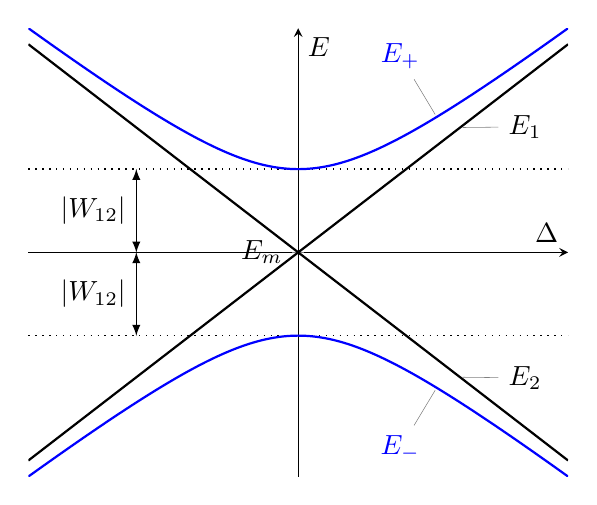
\begin{tikzpicture}
						\begin{axis}
						[
							axis x line=middle,
							axis y line=middle,
							samples=100,
							xlabel=$\Delta$,
							ylabel = $E$,
							ytick = {-1,1},
							yticklabels={,},
							ymajorgrids,
							major y grid style = {line width = 0.5pt,dotted,black},
							xtick = \empty,
							extra y ticks = {1,0},
							extra y tick style = {
								grid=none, 
								yticklabels={,$E_m$},
								yticklabel style={
									yshift=0ex,
									anchor=east
								}
							}
						]
							\addplot[mark=none, thick, smooth] expression { 0.5*x } node [pos=0.8,pin={1:$E_1$},inner sep=0pt] {}; 
							\addplot[mark=none, thick, smooth] expression { -0.5*x } node [pos=0.8,pin={-1:$E_2$},inner sep=0pt] {}; 
							\addplot[mark=none, thick, smooth, color=blue] expression { sqrt(1+(0.5*x)^2)} node [pos=0.75,pin={100:$E_+$},inner sep=0pt] {};
							\addplot[mark=none, thick, smooth, color=blue] expression { -1*sqrt(1+(0.5*x)^2) } node [pos=0.75,pin={-100:$E_-$},inner sep=0pt] {};
							\node (source) at (axis cs:-3,-0.12){};
							\node (destination) at (axis cs:-3,1.12){};
							\draw[latex-latex](source)--(destination);
							\node at (axis cs:-3.8,0.5){$\left|W_{12}\right|$};
 
							\node (source) at (axis cs:-3,0.12){};
							\node (destination) at (axis cs:-3,-1.12){};
							\draw[latex-latex](source)--(destination);
							\node at (axis cs:-3.8,-0.5){$\left|W_{12}\right|$};

						\end{axis}
					\end{tikzpicture}
					\caption{``Anticrossing'' of energy levels}
					\label{fig:anticrossing}
				\end{center}
			\end{figure}
			%
			%

			As one can guess from \figref{anticrossing}, we get an asymptotic behaviour for $|\Delta| \gg |W_{12}|$. For this case, we can approximate the eigenenergies as follows:
			\begin{align}
				E_\pm \approx E_m \pm |\Delta| \left( 1+\frac{1}{2} \left| \frac{W_{12}}{\Delta}\right| ^2+\dots\right).
			\end{align}

			Let us now have a look at the angle $\theta=\arctan(|W_{12}|/\Delta)$ defined previously in \eqref{eq:parameters}. For two different limits, we obtain

			\begin{align}
				\theta \approx \left\{ \begin{array}{lcl} \pm \frac{\pi}{2} & \text{for} & |\Delta| \ll |W_{12}|\\
				0,\pi & \text{for} & |\Delta| \gg |W_{12}| \end{array} \right. 
			\end{align}
			and at $\Delta=0$, we get:
			\begin{align}
				\ket{\psi_\pm}=\frac{1}{\sqrt{2}}\left(\pm \eexp{-i{\varphi}/{2}}\ket{\varphi_1}+ \eexp{i{\varphi}/{2}}\ket{\varphi_2}\right).
			\end{align}
				\paragraph{Examples.} In \figref{twostate}, examples for two-state systems are shown. They can be described quantum-mechanically with a double-well box potential. The single states shown for each system in \figref{twostate} are \emph{not} the eigenstates. In fact, superpositions of the shown states are the eigenstates of the system.

					\begin{figure}
						%\resizebox{\textwidth}{!}{
						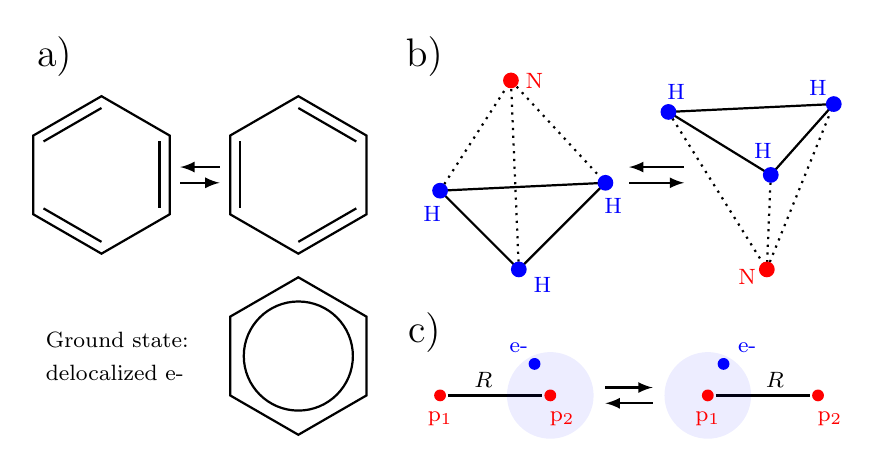
\begin{tikzpicture}

							%%benzene
							\node[align=left] at (-0.6,2.5) {\Large{a)}};
							%left benzene

							\draw[thick] (0 ,0) -- (-{sin(60)} ,{cos(60)}) -- (-{sin(60)} ,{cos(60)+1}) -- (0,{2*cos(60)+1}) -- ({sin(60)} ,{cos(60)+1}) -- ({sin(60)} ,{cos(60)}) -- cycle;

							\draw[thick] (0 , 0.15) -- ({-0.85*sin(60)} ,{0.85*cos(60)+0.15)});

							\draw[thick](-{0.85*sin(60)} ,{1.15*cos(60)+1-0.15}) -- (0,{2*cos(60)+1-0.15});

							\draw[thick] ({sin(60)-0.15*sin(60)} ,{0.85*cos(60)+1}) -- ({sin(60)-0.15*sin(60)} ,{1.15*cos(60)});


							%right benzene

							\draw[thick] (2.5 ,0) -- ({2.5-sin(60)} ,{cos(60)}) -- ({2.5-sin(60)} ,{cos(60)+1}) -- (2.5,{2*cos(60)+1}) -- ({2.5+sin(60)} ,{cos(60)+1}) -- ({2.5+sin(60)} ,{cos(60)}) -- cycle;

							\draw[thick] (2.5,{2*cos(60)+1-0.15}) -- ({2.5+0.85*sin(60)} ,{0.85*cos(60)+1});

							\draw[thick] ({2.5+0.85*sin(60)} ,{0.85*cos(60)+0.15}) -- (2.5 ,0.15);

							\draw[thick] ({2.5-sin(60)+0.15*sin(60)} ,{0.85*cos(60)+1}) -- ({2.5-sin(60)+0.15*sin(60)} ,{1.15*cos(60)});

							%\draw (-{sin(60)} ,{cos(60)}) -- ({sin(60)} ,{cos(60)+1});
							%\draw (-{sin(60)} ,{cos(60)+1}) -- ({sin(60)} ,{cos(60)});
							%\draw (0 ,0) -- (0,{2*cos(60)+1});

							%arrows between the two benzene states

							\draw[-latex,thick](1,{cos(60)+0.4})--(1.5,{cos(60)+0.4});
							\draw[latex-,thick](1,{cos(60)+0.6})--(1.5,{cos(60)+0.6});


							%ground state benzene

							\draw[thick] (2.5 ,-2.3) -- ({2.5-sin(60)} ,{cos(60)-2.3}) -- ({2.5-sin(60)} ,{cos(60)+1-2.3}) -- (2.5,{2*cos(60)+1-2.3}) -- ({2.5+sin(60)} ,{cos(60)+1-2.3}) -- ({2.5+sin(60)} ,{cos(60)-2.3}) -- cycle;

							\draw[thick] (2.5,{cos(60)-1.8}) circle ({0.8*sin(60)});

							\node[align=left] at (0.2,-1.3) {\footnotesize{Ground state:}\\ \footnotesize{delocalized \ch{e-}}};



							%%ammonia
							\node[align=left] at (4.1,2.5) {\Large{b)}};
							%ammonia up

							\draw[thick] (4.3,0.8) -- (5.3,-0.2)  -- (6.4,0.9) -- cycle;
							\draw[thick,dotted] (5.3,-0.2) -- (5.2,2.2);
							\draw[thick,dotted] (4.3,0.8) -- (5.2,2.2) -- (6.4,0.9);

							%\draw[thick] (4,0) -- (5,-1)  -- (6.1,0.1) -- (4.9,1.4) -- cycle;
							%\draw[thick] (5,-1) -- (4.9,1.4);
							%\draw[thick,dashed] (4,0) -- (6.1,0.1);
 
							\fill[fill=blue] (4.3,0.8) circle (0.1);
							\fill[fill=blue] (5.3,-0.2) circle (0.1);
							\fill[fill=blue] (6.4,0.9) circle (0.1);
							\fill[fill=red] (5.2,2.2) circle (0.1);
							\node[color=red] at (5.5,2.2) {\footnotesize{\ch{N}}};
							\node[color=blue] at (4.2,0.5) {\footnotesize{\ch{H}}};
							\node[color=blue] at (5.6,-0.4) {\footnotesize{\ch{H}}};
							\node[color=blue] at (6.5,0.6) {\footnotesize{\ch{H}}};

							%ammonia down

							\draw[thick] (7.2,1.8) -- (8.5,1) -- (9.3,1.9) -- cycle;
							\draw[thick,dotted] (8.5,1) -- (8.45,-0.2);
							\draw[thick,dotted] (7.2,1.8) -- (8.45,-0.2) -- (9.3,1.9); 

							%\draw[thick] (8,1) -- (9.3,0.2)  -- (10.1,1.1) -- (9.25,-1) -- cycle;
							%\draw[thick] (9.3,0.2) -- (9.25,-1);
							%\draw[thick,dashed] (8,1) -- (10.1,1.1);
 
							\fill[fill=blue] (7.2,1.8) circle (0.1);
							\fill[fill=blue] (8.5,1) circle (0.1);
							\fill[fill=blue] (9.3,1.9) circle (0.1);
							\fill[fill=red] (8.45,-0.2) circle (0.1);
							\node[color=red] at (8.2,-0.3) {\footnotesize{\ch{N}}};
							\node[color=blue] at (7.3,2.05) {\footnotesize{\ch{H}}};
							\node[color=blue] at (8.4,1.3) {\footnotesize{\ch{H}}};
							\node[color=blue] at (9.1,2.1) {\footnotesize{\ch{H}}};


							%arrows between ammonia states

							\draw[-latex,thick](6.7,{cos(60)+0.4})--(7.4,{cos(60)+0.4});
							\draw[latex-,thick](6.7,{cos(60)+0.6})--(7.4,{cos(60)+0.6});


							%% H2+ ion
							\node[align=left] at (4.1,-1) {\Large{c)}};
							%electron on right side
							\draw[thick] (4.4,-1.8) -- (5.6,-1.8);
							\fill[fill=blue, opacity=0.07] (5.7,-1.8) circle (0.55);
							\fill[fill=red] (4.3,-1.8) circle (0.075);
							\fill[fill=red] (5.7,-1.8) circle (0.075);
							\fill[fill=blue] (5.5,-1.4) circle (0.075);
							\node[align=right,color=red] at (4.3,-2.1) {\footnotesize{p$_1$}};
							\node[align=left,color=red] at (5.85,-2.1) {\footnotesize{p$_2$}};
							\node[align=right,color=blue] at (5.3,-1.2) {\footnotesize{\ch{e-}}};
							\node[align=right] at (4.85,-1.6) {\footnotesize{$R$}};

							%electron on left side
							\draw[thick] (7.8,-1.8) -- (9.0,-1.8);
							\fill[fill=blue, opacity=0.07] (7.7,-1.8) circle (0.55);
							\fill[fill=red] (7.7,-1.8) circle (0.075);
							\fill[fill=red] (9.1,-1.8) circle (0.075);
							\fill[fill=blue] (7.9,-1.4) circle (0.075);
							\node[align=right,color=red] at (7.7,-2.1) {\footnotesize{p$_1$}};
							\node[align=left,color=red] at (9.25,-2.1) {\footnotesize{p$_2$}};
							\node[align=left,color=blue] at (8.2,-1.2) {\footnotesize{\ch{e-}}};
							\node[align=left] at (8.55,-1.6) {\footnotesize{$R$}};

							%arrows between two electron configuration states
							\draw[-latex,thick](6.4,-1.7)--(7.0,-1.7);
							\draw[latex-,thick](6.4,-1.9)--(7.0,-1.9);
						\end{tikzpicture}
						%}
						\caption{Examples for two-state systems. a) Benzene: In the ground state, the electrons are delocalized. b) Ammonia (\ch{NH3}): The nitrogen atom is either found above or below the hydrogen triangle. The state changes when the nitrogen atom tunnels. c) Molecular ion \ch{H2+}: The electron is either localized near proton p$_1$ or proton p$_2$.}
						\label{fig:twostate}
					\end{figure}

					%\begin{itemize}
					%\item Benzene: Ground state: Delocalized electrons
					%\item Ammonia (\ch{NH3})
					%\item \ch{H2+}
					%\end{itemize}

		\subsection{Dynamical Aspects}
			\subsubsection{Time Evolution of $\ket{\psi(t)}$}
				After the static case we now want to investigate the dynamical properties of the two-state system. We calculate the time evolution of $\ket{\psi(t)} = \left(\begin{array}{cc} a_1(t) & a_2(t)\end{array}\right)^T$ with the Schrödinger equation and the perturbed Hamiltonian \eqref{eq:perturbedhamiltonian}:
				\begin{align}
					i\hbar \diff{}{t}\ket{\psi(t)}&=\left(\hat{H}+\hat{W}\right)\ket{\psi(t)},\\
					i\hbar \diff{}{t}\left(\begin{array}{c} a_1(t) \\ a_2(t) \end{array}\right) &= \left( \begin{array}{cc} \tilde{E}_1 & W_{12} \\ W_{12}^* & \tilde{E}_2 \end{array} \right) \left(\begin{array}{c} a_1(t) \\ a_2(t) \end{array} \right).
				\end{align}
				For the state $\ket{\psi(t)}$ we get
				\begin{align}
					\ket{\psi(t)}=\lambda \eexp{-i{E_+}t/{\hbar}} \ket{\psi_+} + \mu \eexp{-i{E_-}t/{\hbar}} \ket{\psi_-} \label{eq:psitimeevolution}
				\end{align}
				with the factors $\lambda$ and $\mu$.

				If we start in the state $\ket{\varphi_1}$, what is the probability
				\begin{align}
					P_2(t)=\left|\braket{\varphi_2|\psi(t)}\right|^2
				\end{align}
				to find the system in the state $\ket{\varphi_2}$? As a first step, we have to apply the initial condition to \eqref{eq:psitimeevolution} and express $\ket{\varphi}$ in terms of \eqref{eq:staticpsiplus} and \eqref{eq:staticpsiminus}:
				\begin{align}
					\ket{\psi(0)} \overset{!}{=}& \ket{\varphi_1}\\
											  = & \eexp{i{\varphi}/{2}} \left[ \cos\left( \frac{\theta}{2}\right) \ket{\psi_+}-\sin\left(\frac{\theta}{2}\right)\ket{\psi_-}\right]
				\end{align}
				By equating the coefficients we get for $\lambda$ and $\mu$:
				\begin{align}
					\lambda = \eexp{i{\varphi}/{2}}\cos\left(\frac{\theta}{2}\right), \qquad  \mu = -\eexp{i{\varphi}/{2}}\sin\left(\frac{\theta}{2}\right).
				\end{align}
				One thus gets:
				\begin{align}
					\hspace{-2mm} P_2(t)	=&\left|\braket{\varphi_2|\psi(t)}\right|^2 \\
											=& \left|\eexp{i\varphi} \sin\left(\frac{\theta}{2}\right)\cos\left(\frac{\theta}{2}\right)\left[\eexp{-i{E_+}t/{\hbar}} - \eexp{-i{E_-}t/{\hbar}}\right]\right|^2\\
											=& \sin^2(\theta)\sin^2\left(\frac{E_+-E_-}{2\hbar}t\right)
				\end{align}
				$P_2(t)$ can be expressed with $\Delta$ and $W_{12}$ alone. The obtained relation is called Rabi's formula:
				\begin{align}
					\Aboxed{P_2(t)=\frac{1}{1+\left(\frac{\Delta}{|W_{12}|}\right)^2}\sin^2\left(\sqrt{|W_{12}|^2+\Delta^2}\frac{t}{\hbar}\right)}
				\end{align}

				\begin{figure}
					\begin{center}
						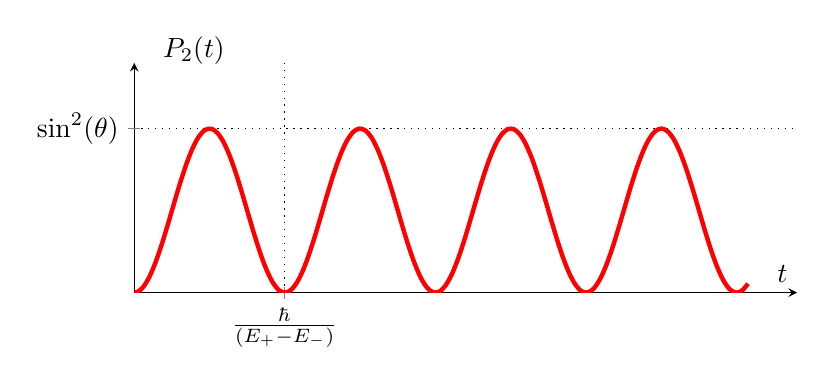
\begin{tikzpicture}
							\begin{axis}
							[
								axis x line=middle,
								axis y line=left,
								xmin = 0, xmax = {5.4},
								ymin = 0, ymax = {1.4},
								samples=200,
								xlabel=$t$,
								y label style={at={(axis description cs:0.09,.95)},rotate=-90,anchor=south},
								ylabel = $P_2(t)$,
								xtick = \empty,
								ytick = \empty,
								height = 4.5cm,
								width = 10cm,
								extra x ticks = {1.225},
								extra y ticks = {1},
								extra tick style={grid=major, grid style={line width = 0.5pt, dotted, black}},
								extra x tick labels={$\frac{\hbar}{(E_+-E_-)}$},
								extra y tick labels={$\sin^2(\theta)$},
							]
							\addplot[mark=none, ultra thick, smooth, color=red] expression {(sin(46.7*x*pi))^2};
							\end{axis}
						\end{tikzpicture}
						\caption{Rabi oscillations}
					\end{center}
				\end{figure}
\marginpar{\scriptsize{Lecture 4}}
	\section{Two-Level System in an Oscillatory Field}
		An atom has many energy levels $E_n$ and most of them are degenerate. How can we reduce this complicated structure to a two-level system?
		The solution is to resonantly couple two of the atom's levels by applying an external, oscillatory field.

		\subsection[Time-Dependent Perturbation Theory]{Time-Dependent Perturbation Theory\footnote{cf. \cite{basdevant}, chapter 12}} \label{sec:tdperturbationtheory}
			For the atom in the oscillatory field we can write down the Hamiltonian:

			\begin{align}
				\hat{H} = \hat{H}_0 + \hat{H}_1(t).
			\end{align}
			Here, $\hat{H}_0$ belongs to the atom and $\hat{H}_1(t)$ describes the time-dependent field and its interaction with the atom.
			We assume that $\ket{n}$ is an eigenstate of $\hat{H}_0$ and write:
			%
			\begin{align}
				\hat{H}_0\ket{n} = E_n \ket{n}.
			\end{align}
			
			If the system is initially prepared in the state $\ket{n}$, so that
			\begin{align}
				\ket{\psi(t=0)} = \ket{n},
			\end{align}
			what is the probability
			\begin{align}
				P_m(t) \coloneqq \left|\braket{m|\psi(t)}\right|^2
			\end{align}
			to find the system in the state $\ket{m}$ at the time $t$?

			\subsubsection{Evolution Equation}
				The system $\ket{\psi(t)}$ can be expressed as follows:
				\begin{align}
					\ket{\psi(t)} = \sum_n \gamma_n(t) \eexp{-i{E_n}t/{\hbar}} \ket{n},
				\end{align}
				where the exponential is the time evolution for $\hat{H}_1 =~0$.
				We plug this equation in the Schrödinger equation and get:
				\begin{multline}
					\hphantom{\Longleftrightarrow} i\hbar \sum_n\left(\dot{\gamma}_n(t)-i\frac{E_n}{\hbar}\gamma_n(t)\right)\eexp{-i{E_n}t/{\hbar}}\ket{n} \\
					= \sum_n \gamma_n(t) \eexp{-i{E_n}t/{\hbar}}\left(\hat{H}_0 + \hat{H}_1\right) \ket{n}
				\end{multline}
				\begin{multline}\label{eq:timeev}
					\Longleftrightarrow i\hbar\sum_n \dot{\gamma}_n(t) \eexp{-i{E_n}t/{\hbar}} \ket{n}\\
					= \sum_n \gamma_n(t) \eexp{-i{E_n}t/{\hbar}} \hat{H}_1 \ket{n}
				\end{multline}
				%
				If we multiply \eqref{eq:timeev} with $\bra{k}$ we obtain a set of coupled differential equations
				\begin{align}
					i\hbar \dot{\gamma}_k \eexp{-i{E_k}t/{\hbar}} &= \sum_n \gamma_n \eexp{-{E_n}t/{\hbar}}\bra{k}\hat{H}_1\ket{n},\\
					i\hbar \dot{\gamma}_k &= \sum_n \gamma_n \eexp{-i {(E_n-E_k)}t/{\hbar}} \bra{k} \hat{H}_1\ket{n}
				\end{align}
				with initial conditions $\ket{\psi(t=0)}$. They determine the full time evolution.

			\subsubsection{Perturbative Solution}
				We assume that
				\begin{align}
					\hat{H}_\lambda = \hat{H}_0 + \lambda \hat{H}_1(t),
				\end{align}
				where $\lambda$ is a small parameter. We expand
				\begin{align}
					\gamma_n(t) = \gamma_n^{(0)} + \lambda \gamma_n^{(1)} + \lambda^2 \gamma_n^{(2)} + \dots
				\end{align}
				and plug this ansatz in the evolution equations and sort them by terms of equal power in $\lambda$:
				The $0$th order reads
				\begin{align}
					i\hbar \dot{\gamma}_k^{(0)} = 0,
				\end{align}
				and for the $1$st order we get
				\begin{align} \label{eq:1storderapprox}
					i\hbar \dot{\gamma}_k^{(1)} = \sum_n \gamma_n^{(0)}(t) \eexp{-i(E_n-E_k)t/{\hbar}}\bra{k}\hat{H}_1\ket{n}.
				\end{align}
				The $0$th order does not have a time evolution since it is the initial state.

			\subsubsection{First Order Solution (Born Approximation)}
For the initial conditions $\psi(t=0)=\ket{i}$ we get
\begin{align}
\gamma_k^{(0)}(t) = \delta_{ik}.
\end{align}
We plug this in the $1$st order approximation \eqref{eq:1storderapprox} and obtain the rate for the system to go to the final state $\ket{f}$:
%
\begin{align}
i \hbar\dot{\gamma}^{(1)} = \eexp{i(E_f-E_i)t/{\hbar}} \bra{f}\hat{H}_1 \ket{i}
\end{align}
Integration with $\gamma_f^{(1)}(t=0) = 0$ yields
\begin{align}\label{eq:gammaf1}
\Aboxed{\gamma_f^{(1)} = \frac{1}{i\hbar}\int\limits_0^t \eexp{i(E_f-E_i)t'/{\hbar}} \bra{f} \hat{H}_1(t')\ket{i} \dif t',}
\end{align}
so that we obtain the probability for ending up in the final state:
\begin{align}
P_{i\to f}(t) = \left| \gamma_f^{(1)}(t)\right|^2.
\end{align}
Note that  $ P_{i\to f}(t) \ll 1$ is the condition for this approximation to be valid!
\paragraph{Example 1: Constant Perturbation.}
\begin{figure}
\begin{center}
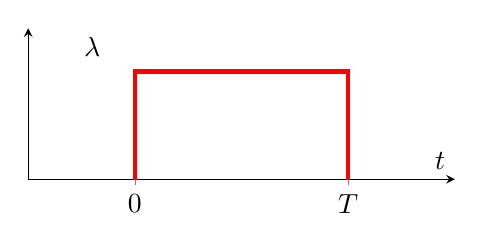
\begin{tikzpicture}
\begin{axis}
[
	axis x line=middle,
	axis y line=left,
	xmin = {0}, xmax = {4},
	ymin = 0, ymax = {1.4},
	samples=200,
	xlabel=$t$,
	y label style={at={(axis description cs:0.15,.75)},rotate=-90,anchor=south},
	ylabel = $\lambda$,
	xtick = \empty,
	ytick = \empty,
	height = 3.5cm,
	width = 7cm,
	extra x ticks = {1,3},
%	extra y ticks = {1},
%	extra tick style={grid=major, grid style={dotted, cyan}},
	extra x tick labels={$0$,$T$},
%	extra y tick labels={$\omega_0$},
]
 \node (source) at (axis cs:1,-0.13){};
 \node (destination) at (axis cs:3,-0.13){};
 \draw[-, color=red,ultra thick](source)-- (axis cs:1,1) -- (axis cs:3,1) -- (destination);
\end{axis}
\end{tikzpicture}
\caption{Sketch of a constant perturbation}
\label{fig:constpert}
\end{center}
\end{figure}
We apply a constant perturbation in the time interval $\left[0,T\right]$, as shown in \figref{constpert}. If we use \eqref{eq:gammaf1} and set $\hbar \omega_0 = E_f-E_i$, we get
\begin{align}
\gamma_f^{(1)}(t\geq T) = \frac{1}{i \hbar} \bra{f}\hat{H}_1\ket{i} \frac{\eexp{i\omega_0 T}-1}{i\omega_0},
\end{align}
and therefore
\begin{align}
P_{i\to f} = \frac{1}{\hbar^2}\left|\bra{f}\hat{H}_1\ket{i}\right|^2 \underbrace{\frac{\sin^2\left(\omega_0\frac{T}{2}\right)}{\left(\frac{\omega_0}{2}\right)^2}}_{\operatorname{y}(\omega_0,T)}.
\end{align}
A sketch of $\operatorname{y}(\omega_0,T)$ is shown in \figref{sinc}.

\begin{figure}
\begin{center}
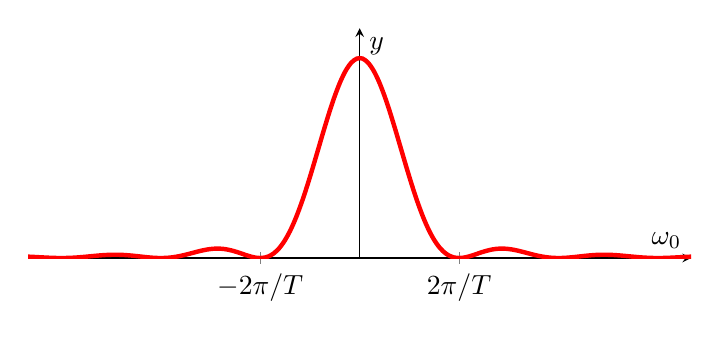
\begin{tikzpicture}
\begin{axis}
[
	axis x line=middle,
	axis y line=center,
	xmin = {-3}, xmax = {3},
	ymin = 0, ymax = {1.4},
	samples=200,
	xlabel=$\omega_0$,
%	y label style={at={(axis description cs:0.09,.95)},rotate=-90,anchor=south},
	ylabel = $\operatorname{y}$,
	xtick = \empty,
	ytick = \empty,
	height = 4.5cm,
	width = 10cm,
	extra x ticks = {-0.9,0.9},
%	extra y ticks = {1},
%	extra tick style={grid=major, grid style={dotted, cyan}},
	extra x tick labels={$-2\pi/T$,$2\pi/T$},
%	extra y tick labels={$\omega_0$},
]
	\addplot[mark=none, ultra thick, smooth, color=red] expression {((sin(200*x)/(x))^2)/10};
\end{axis}
\end{tikzpicture}
\caption{A sketch of $\operatorname{y}(\omega_0,T)$}
\label{fig:sinc}
\end{center}
\end{figure}


\paragraph{Example 2: Sinusoidal Perturbation.}
For the perturbation
\begin{align}
\hat{H}_1(t) = \left\{ \begin{array}{ccl} \hat{H}_1\eexp{-i\omega t} && \text{for}\; 0 < t < T \\ 0 &&\text{otherwise}\end{array} \right.
\end{align}
we obtain the probability
\begin{align}
P_{i\to f} (t \geq T) = \frac{1}{\hbar^2} \left|\bra{f}\hat{H}_1\ket{i}\right|^2 \operatorname{y}(\omega_0 - \omega, T).
\end{align}
%
At $\omega = \left|E_f - E_i\right|/\hbar$ we are on resonance.

\subsection[Rabi Oscillation]{Rabi Oscillation\footnote{cf. \cite{basdevant}, chapter 12.5}}
As an example we consider the magnetic moment of a spin $1/2$ in an oscillating magnetic field
\begin{align}
\vec{B}(t) = B_0 \vec{e}_z + B_1 (\cos(\omega t) \vec{e}_x+ \sin(\omega t) \vec{e}_y).
\end{align}
The Hamiltonian then reads:
\begin{align}
\hat{H} &= - \hat{\vec{\mu}}\cdot\vec{B}(t)\\ 
		&= -\mu_B (B_0 \hat{\sigma}_z + B_1(\cos(\omega t) \hat{\sigma}_x + \sin(\omega t) \hat{\sigma}_y)
\end{align}
In the matrix form we get:
\begin{align}
\hat{H} = -\mu_0 \left( \begin{array}{cc} B_0 & B_1 \overbrace{(\cos(\omega t) - i \sin(\omega t))}^{\eexp{-i\omega t}} \\ B_1 \underbrace{(\cos(\omega t) + i \sin(\omega t))}_{\eexp{i\omega t}} & -B_0 \end{array} \right).
\end{align}
If we define $\hbar \omega_0 = 2 \mu_B \cdot B_0$ and $\hbar\omega_1 = 2 \mu_B \cdot B_1$, the matrix form becomes
\begin{align} \label{eq:matrixbfield}
\hat{H} = \frac{1}{2}\hbar \left( \begin{array}{cc} -\omega_0 & \omega_1 \eexp{-i\omega t}\\ \omega_1 \eexp{i\omega t } & \omega_0 \end{array} \right)
\end{align}
We plug \eqref{eq:matrixbfield} in the Schrödinger equation
\begin{align}
i\hbar \diffp{}{t} \left(\begin{array}{cc}a_+(t)\\ a_-(t) \end{array} \right) = \hat{H} \left(\begin{array}{c}a_+(t) \\ a_-(t) \end{array} \right)
\end{align}
and obtain
\begin{align}
i \dot{a}_+(t) = \frac{\omega_0}{2} a_+(t) + \frac{\omega_1}{2} \eexp{-i\omega t} a_-(t),\\
i \dot{a}_-(t) = -\frac{\omega_0}{2}a_-(t) + \frac{\omega_1}{2}\eexp{i\omega t}a_+(t).
\end{align}
%
Lastly, we transform into the ``rotating frame'' by defining
\begin{align}
b_\pm (t) \coloneqq \eexp{\pm i \omega {t}/{2}} a_\pm (t),
\end{align}
which yields
\begin{align}
i\dot{b}_+ &=-	\frac{\omega-\omega_0}{2}b_+ + \frac{\omega_1}{2}b_-,\\
i\dot{b}_- &=\hphantom{-}\frac{\omega - \omega_0}{2} b_- + \frac{\omega_1}{2}b_+
\end{align}
and therefore a time-independent Hamiltonian
\begin{align}
\hat{H}' = \frac{\hbar}{2} \left( \begin{array}{cc} -(\omega-\omega_0) & \omega_1 \\ \omega_1 & (\omega-\omega_0) \end{array} \right).